%%%%%%%%%%%%%%%%%%%%%%%VICARIOUS%%%%%%%%%%%%%%%%%%%%%%%%%%%%%%%%%%%%%%%
% Copyright ME, FUCK YOU												%
% Template for presentation in Latex`s Beamer Class					%
% Using the default Berlin theme, can be replaced by other themes		%
% logo in the upper right can be replaced by new .png, gif, eps etc	%
% 																		%
%%%%%%%%%%%%%%%%%%%%%%%%%%%%%%%%%%%%%%%%%%%%%%%%%%%%%%%%%%%%%%%%%%%%%%%
\documentclass[xcolor=dvipsnames,aspectratio=169]{beamer}
\usetheme{Berlin}
\usecolortheme[named=LimeGreen]{structure}
\usepackage{beamerthemesplit} % kam neu dazu
\usepackage[ngerman]	{babel}			
\usepackage{t1enc}						
\usepackage[utf8]{inputenc}			
\usepackage{amsmath}
\usepackage{graphicx}
\graphicspath{{pictures/}}
\usepackage{amssymb}
\usepackage{amsfonts}
\usepackage{caption}
\usepackage{multimedia}
\usepackage{tikz}
\usepackage{listings}
\usepackage{acronym}

\usepackage{lmodern}
\usepackage{multicol}


\definecolor{pblue}{rgb}{0.13,0.13,1}
\definecolor{pgreen}{rgb}{0,0.5,0}
\definecolor{pred}{rgb}{0.9,0,0}
\definecolor{pgrey}{rgb}{0.46,0.45,0.48}

\lstset{
    escapeinside={(*}{*)}
}

\lstdefinestyle{Java}{
  showspaces=false,
  showtabs=false,
  tabsize=2,
  breaklines=true,
  showstringspaces=false,
  breakatwhitespace=true,
  commentstyle=\color{pgreen},
  keywordstyle=\color{pblue},
  stringstyle=\color{pred},
  basicstyle=\footnotesize\ttfamily,
  numbers=left,
  numberstyle=\tiny\color{gray}\ttfamily,
  numbersep=7pt,
  %moredelim=[il][\textcolor{pgrey}]{$$},
  moredelim=[is][\textcolor{pgrey}]{\%\%}{\%\%},
  captionpos=b
}

\lstdefinestyle{basic}{  
  basicstyle=\footnotesize\ttfamily,
  breaklines=true
  numbers=left,
  numberstyle=\tiny\color{gray}\ttfamily,
  numbersep=7pt,
  backgroundcolor=\color{white},
  showspaces=false,
  showstringspaces=false,
  showtabs=false,
  frame=single,
  rulecolor=\color{black},
  captionpos=b,
  keywordstyle=\color{blue}\bf,
  commentstyle=\color{gray},
  stringstyle=\color{green},
  keywordstyle={[2]\color{red}\bf},
}


\lstdefinelanguage{custom}
{
morekeywords={public, void},
sensitive=false,
morecomment=[l]{//},
morecomment=[s]{/*}{*/},
morestring=[b]",
}


\lstdefinestyle{BashInputStyle}{
  language=bash,
  showstringspaces=false,
  basicstyle=\small\sffamily,
  numbers=left,
  numberstyle=\tiny,
  numbersep=5pt,
  frame=trlb,
  columns=fullflexible,
  backgroundcolor=\color{gray!20},
  linewidth=0.9\linewidth,
  xleftmargin=0.1\linewidth
}

%Logo in the upper right just change if you know what you are doing^^
\addtobeamertemplate{frametitle}{}{%
\begin{tikzpicture}[remember picture,overlay]
\node[anchor=north east,yshift=2pt] at (current page.north east) {
\includegraphics[height=1.8cm]{htw}};
\end{tikzpicture}}

\begin{document}
\bibliographystyle{alpha}
\title{Netzwerke -- Seminaristische Übung WS17/18}
\subtitle{Grundlagen *nix \& Shell\\
\href{mailto:Benjamin.Troester@HTW-Berlin.de}{Benjamin.Troester@HTW-Berlin.de}\\
		PGP: ADE1 3997 3D5D B25D 3F8F 0A51 A03A 3A24 978D D673 }
\author{Benjamin Tröster}

\date{\today}

\begin{frame}
\titlepage
\end{frame}

\section*{Road-Map}
\begin{frame}
\frametitle{Road-Map}
\begin{multicols}{2}
  \tableofcontents
\end{multicols}
\end{frame}

\section{Labor}
\subsection{Laborrechner \& Infrastruktur}
\begin{frame}
\begin{itemize}
	\item WH C 625
	\item 21 Dell Optiplex
	\begin{itemize}
		\item Intel i7-7700
		\item 16 GB RAM
		\item 256 GB SATA-SSD
		\item Ubuntu 16.04 / Windows 10
	\end{itemize}
	\item GBit-\ac{lan}
	\item GBit-\ac{wan} ins \ac{dfn}
\end{itemize}
\end{frame}

\subsection{Raspberry Pi}
\begin{frame}
\begin{itemize}
	\item Raspberry Pi -- \ac{soc}
	\item Architektur: ARMv6Z (32-bit)
	\item 700 MHz 1 Core  ARM11
	\item 512 MB RAM
	\item 10/100 Mbit/s Ethernet
	\item Raspbian 9 Stretch -- Debian Fork
\end{itemize}
\end{frame}

\section{Unixoide}
\subsection{Historisches zu Unix}

\begin{frame}
 \begin{tabular}{lc}
 \hspace*{-1.3cm} 
 \parbox{0.65\linewidth}{
\begin{itemize}
	\item Eigentlich von \ac{unics} als Anspielung auf Multics
	\item 1969 entwickelt in den Bell Laboratories
	\item Bekannte Vertreter:
	\begin{itemize}
	\item \ac{bsd}, SunOS/ Solaris, Minix
	\end{itemize}
\end{itemize} } 
& \begin{tabular}{l}
 \begin{tabular}{c}
 \hspace*{-1.1cm}
           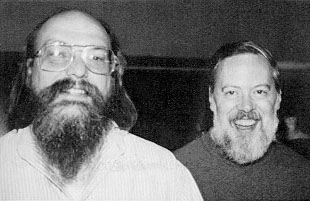
\includegraphics[scale=0.45]{Ken_n_dennis}
           \end{tabular}
\end{tabular}\\
\end{tabular}
\end{frame}

\begin{frame}
\begin{figure}
 \vspace*{-.5cm} 
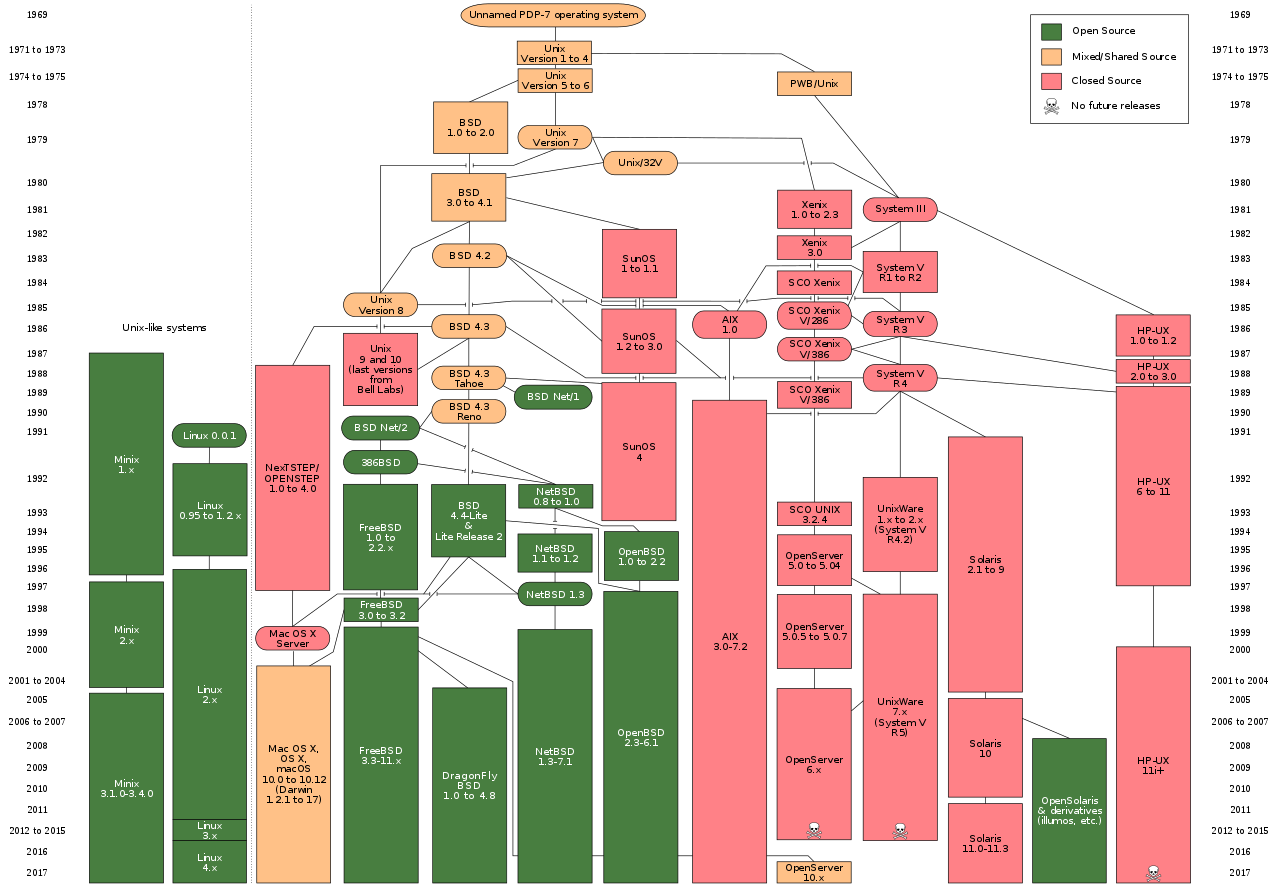
\includegraphics[scale=0.24]{unix_hist}
\end{figure}
\end{frame}

\subsection{Linux}

\begin{frame}
 \begin{tabular}{lc}
 \hspace*{-1.3cm} 
 \parbox{0.65\linewidth}{
\begin{itemize}
	\item 1991 im Usenet veröffentlicht von Linus Torvalds
	\item Linux im wesentlichen Kernel + GNU-Tools
	\item Distributionen nutzen (angepassten) Linux Kernel + (eigene) Standardsoftware, wie Paketmanager etc
	\item Bekannte Linux Distributionen:
	\begin{itemize}
	\item Slackware, Red Hat, Debian, Gentoo, Arch Linux
	\end{itemize}
\end{itemize} } 
& \begin{tabular}{l}
 \begin{tabular}{c}
 \hspace*{-0.5cm}
           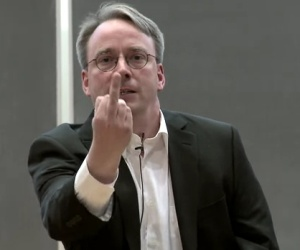
\includegraphics[scale=0.5]{linus}
           \end{tabular}
\end{tabular}\\
\end{tabular}
\end{frame}

\subsection{Aufbau Linux}
\begin{frame}
 \begin{tabular}{lc}
 \hspace*{-1.3cm} 
 \parbox{0.65\linewidth}{
\begin{itemize}
	\item Hardware
	\begin{itemize}
		\item CPU, RAM, Mainboard ...
	\end{itemize}
	\item Kernel -- Betriebssystemkern
	\begin{itemize}
		\item Gerätetreiber, Dateisystem, Prozessteuerung, Systemaufrufe ...
	\end{itemize}
	\item Shell -- Schnittstelle zwischen Nutzer \& Diensten des Betriebssystems
	\begin{itemize}
		\item \ac{cli} oder \ac{gui}
		\item Interpretiert \& bearbeitet Eingaben des Nutzers
	\end{itemize}
	\item Anwendungsprogramme
	\begin{itemize}
		\item Standardsoftware des Betriebssystems \& 3rd-Party-Software
	\end{itemize}

\end{itemize} } 
& \begin{tabular}{l}
 \begin{tabular}{c}
 \hspace*{-1cm}
           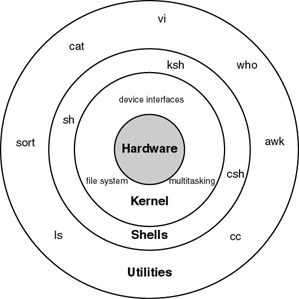
\includegraphics[scale=0.5]{unix_arch}
           \end{tabular}
\end{tabular}\\
\end{tabular}
\end{frame}

\subsection{Aufbau Filesystem}
\begin{frame}
\begin{figure}
 %\hspace*{-0.5cm}
  \vspace*{-0.3cm}
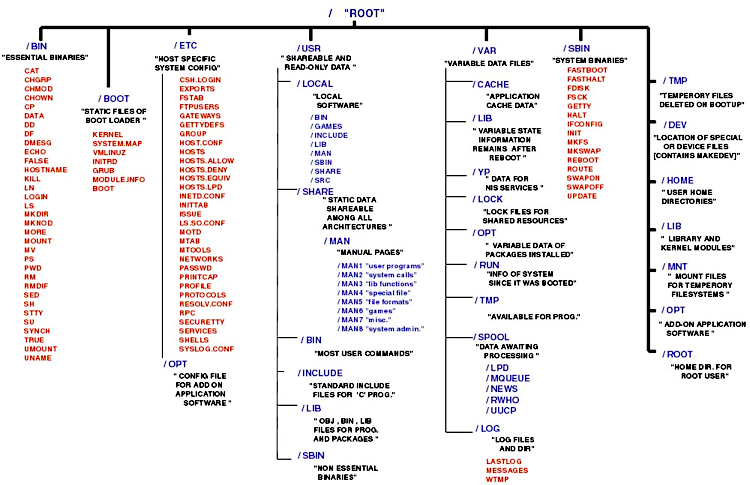
\includegraphics[scale=0.4]{filesystem}
\end{figure}
\end{frame}

\begin{frame}
In Linux/ Unix ist grundsätzlich alles eine Datei!\\
\textbf{Baumstruktur -- statt separate Laufwerke/ Massenspeicher}
Exemplarisch:
\begin{itemize}
	\item / -- Wurzelverzeichnis
	\item /bin -- wichtigste Programme in Binäreformat
	\item /boot -- Boot-Loader
	\item /etc -- System Konfiguration

	\item /usr -- Konfiguration, Shared-Software
	\begin{itemize}
		\item /usr/local -- lokale Software
		\item /usr/share -- statische Daten
		\item /usr/bin -- User-Land-Software/ Commands
		\item /usr/include -- Standard-Bibliotheken für C/C++
		\item /usr/lib -- Bibliotheken für Programmiersprachen
		\item /usr/sbin -- andere Binaries
	\end{itemize}

\end{itemize}
\end{frame}
\begin{frame}
\begin{itemize}
\item /var -- Variable Daten
	\begin{itemize}
		\item /var/log -- zentrale Log-File-Stelle
	\end{itemize}
	\item /sbin -- System Binaries
	\item /tmp -- Temporäre Dateien
	\item /dev -- Geräte
	\item /home -- User-Bereich
	\item /lib -- Bibliotheken \& Kernel-Module
	\item /opt -- zustätzliche Software -- Add Ons
	\item /root -- Verzeichnis vom Root-User
\end{itemize}
Ausführlicher: \url{https://en.wikipedia.org/wiki/Unix_filesystem\#Conventional_directory_layout}
\end{frame}

\subsection{User, Gruppen}
\begin{frame}
Linux/ Unix sind Mehrbenutzersysteme, d.h. mehrere Nutzer können simultan auf einem Rechner arbeiten
\begin{itemize}
	\item Zuordnung der Nutzer zu User \& Group
	\item Regelt Zugangskontrolle im System auf
	\begin{itemize}
	\item  Dateien, Ordner \& Peripheriegeräte
	\end{itemize}
	\item Unterschiedliche Nutzer/ Gruppen $\rightarrow$ unterschiedliche Rechte
	\item Im Labor:
	\begin{itemize}
		\item Benutzername: Matrikelnummer
		\item Gruppen: student, domain, users
	\end{itemize}
	\item Raspberry Pi:
	\begin{itemize}
		\item Benutzername: pi
		\item Gruppen: users, wheel
	\end{itemize}
\end{itemize}
\end{frame}

\subsection{Nutzerrechte}
\begin{frame}
Um die Zugriffsrechte der jeweiligen Nutzer zu regeln bietet Linux/ Unix ein Berechtigungsmodell\\
Abbildung der Nutzer, Gruppen auf Zugriffsmöglichkeiten der Dateien
\begin{itemize}
	\item Grundsätzlich in drei Kategorien:
	\begin{itemize}
		\item Owner -- regelt Berechtigung des Eigentümers
		\item Group -- regelt Berechtigung der Gruppe
		\item Other (world) -- regelt Berechtigung aller anderen Nutzer 
	\end{itemize}
	\item Unix Zugriffsmodi:
	\begin{itemize}
		\item read (r) -- Lesezugriff
		\item write (w) -- Schreibzugriff
		\item execute (x) -- Ausführzugriff
	\end{itemize}
\end{itemize}
\end{frame}

\begin{frame}
Zahlensystem:
\begin{itemize}
	\item Dezimalsystem -- Basis 10
	\begin{itemize}
		\item Werte 0 - 9 
	\end{itemize}
	\item Dualsystem/ Binärsystem -- Basis 2
	\begin{itemize}
		\item Werte 0 oder 1
		\item Bit-Darstellung in der Informatik/ Rechnertechnik
	\end{itemize}
	\item Oktalsystem -- Basis 8
	\begin{itemize}
		\item Werte 0 - 7
		\item Für Darstellung der Zahlen 0 - 7 $\rightarrow$ 3 Bit notwendig, $2^3 = 8$
	\end{itemize}
\end{itemize}
\end{frame}


\begin{frame}
Darstellung im System via Oktalzahlen:
\begin{itemize}
	\item Zuordnung der Berechtigung r,w,x bestimmten Werten
	\begin{itemize}
		\item Lesen (r) $\rightarrow$ $4_8$ oder $100_2$
		\item Schreiben (w) $\rightarrow$ $2_8$ oder $010_2$
		\item Ausführen (x) $\rightarrow$ $1_8$ oder $001_2$
		\item None $\rightarrow$ $0_8$ oder $000_2$
	\end{itemize}
	\item Zusammensetzen der Oktalwerte ergibt Zugriffsrechte:
	\begin{itemize}
		\item Lesen, schreiben und ausführen $\rightarrow$ $7_8$ oder $111_2$
		\item Lesen und Schreiben $\rightarrow$ $6_8$ oder $110_2$
		\item Lesen und Ausführen $\rightarrow$ $5_8$ oder $101_2$
		\item ...
	\end{itemize}
\end{itemize}
\end{frame}

\begin{frame}
Zusammensetzung der Berechtigung
\begin{itemize}
	\item 3er-Oktett gibt Zugriffmodalitäten an
	\begin{enumerate}
		\item User r,w,x -- erstes Oktett
		\item group r,w,x -- zweites Oktett
		\item other r,w,x -- drittes Oktett
	\end{enumerate}
\end{itemize}
\begin{figure}
	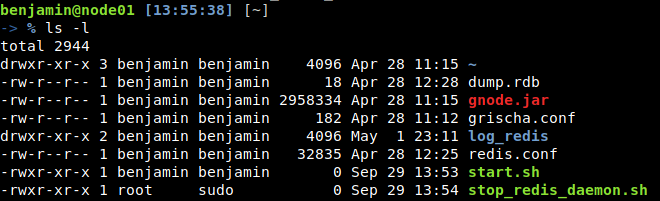
\includegraphics[scale=0.5]{rights}
\end{figure}
\end{frame}

\section{Shell}

\subsection{Einführung}

\subsection{Commands}

\subsection{Anlaufstellen}

\section{Filesystem}

\begin{acronym}
\acro{bsd}[BSD]{Berkeley Software Distribution}
\acro{cli}[CLI]{Command Line Interface}
\acro{dfn}[DFN]{Deutsches Forschungsnetz}
\acro{gui}[GUI]{Graphical User Interface}
\acro{gw}[GW]{Gateway}
\acroplural{gws}[GW`s]{Gateways}
\acro{lan}[LAN]{Local Area Network}
\acro{moco}[MOCO]{Mobile Computing}
\acro{soc}[SoC]{System on a chip}
\acro{wan}[WAN]{Wide Are Network}
\acro{unics}[UNICS]{Uniplexed Information and Computing Service}
\end{acronym}

\end{document}